% Preamble
\documentclass{beamer}
\usetheme{Singapore}
\usecolortheme{seahorse}
\usepackage{graphicx, wrapfig, subcaption, setspace, booktabs}
\usepackage[T1]{fontenc}
\usepackage[font=small, labelfont=bf]{caption}
\usepackage{fourier}
\usepackage{url, lipsum}
\usepackage{enumerate}
\usepackage{mdframed}
\usepackage{soul}
\usepackage{xcolor}
\usepackage{amsmath}
\usepackage{amssymb}

% Theme selection

% Title page setup
\title[Superscalar Fixed-Length Vector Processor]{ECE-5580 Computer Architecture: Final Project} % Project title
\subtitle{Superscalar Fixed-Length Vector Pipeline} % Project subtitle
\author[Garza et al.]{Dylan-Matthew Garza \and Elijah Sargeant} % Student names
\institute[Western Michigan University]{ % University and department name
  Department of Electrical and Computer Engineering \\
  Western Michigan University 
}
\date{\today} % Date, can be changed to a specific date
%\logo{\includegraphics[height=1cm]{university-logo.png}} % University logo

% Document body
\begin{document}

% Cover slide
\begin{frame}
  \titlepage % This command inserts the title page
\end{frame}

% Table of contents (optional)
\begin{frame}{Table of Contents}
  \tableofcontents % You can add sections and subsections to auto-populate
\end{frame}

% Section 1
\section{Idea and Implementation}
\begin{frame}{Background on Vector Processors}
    \subsection{Background on Vector Processors}
    \begin{itemize}
        \item Vector architectures implement SIMD
            (Single Instruction Multiple Data) by operating 
            on sequential register files that contain multiple elements.
        \item Increases performance by reducing the total number of instructions
            needed on repeated computations.
        \item Vector architectures usually are not standalone implementations in 
            modern applications and usually are implemented in MME 
            (Multimedia Extensions):
            \begin{itemize}
                \item Intel's AVX (Advanced Vector Extensions) \& 
                    AMD's SSE (Streaming SIMD Extensions)
                \item GPUs (SIMD with vector operations)
            \end{itemize}
        \item Intel and AMD vector extension's support fixed-vectors
    \end{itemize}
\end{frame}

% Section 2
\section{Initial Planned Implementation}
\subsection{High Level Overview}
\begin{frame}{Implementation}
    \begin{center}
    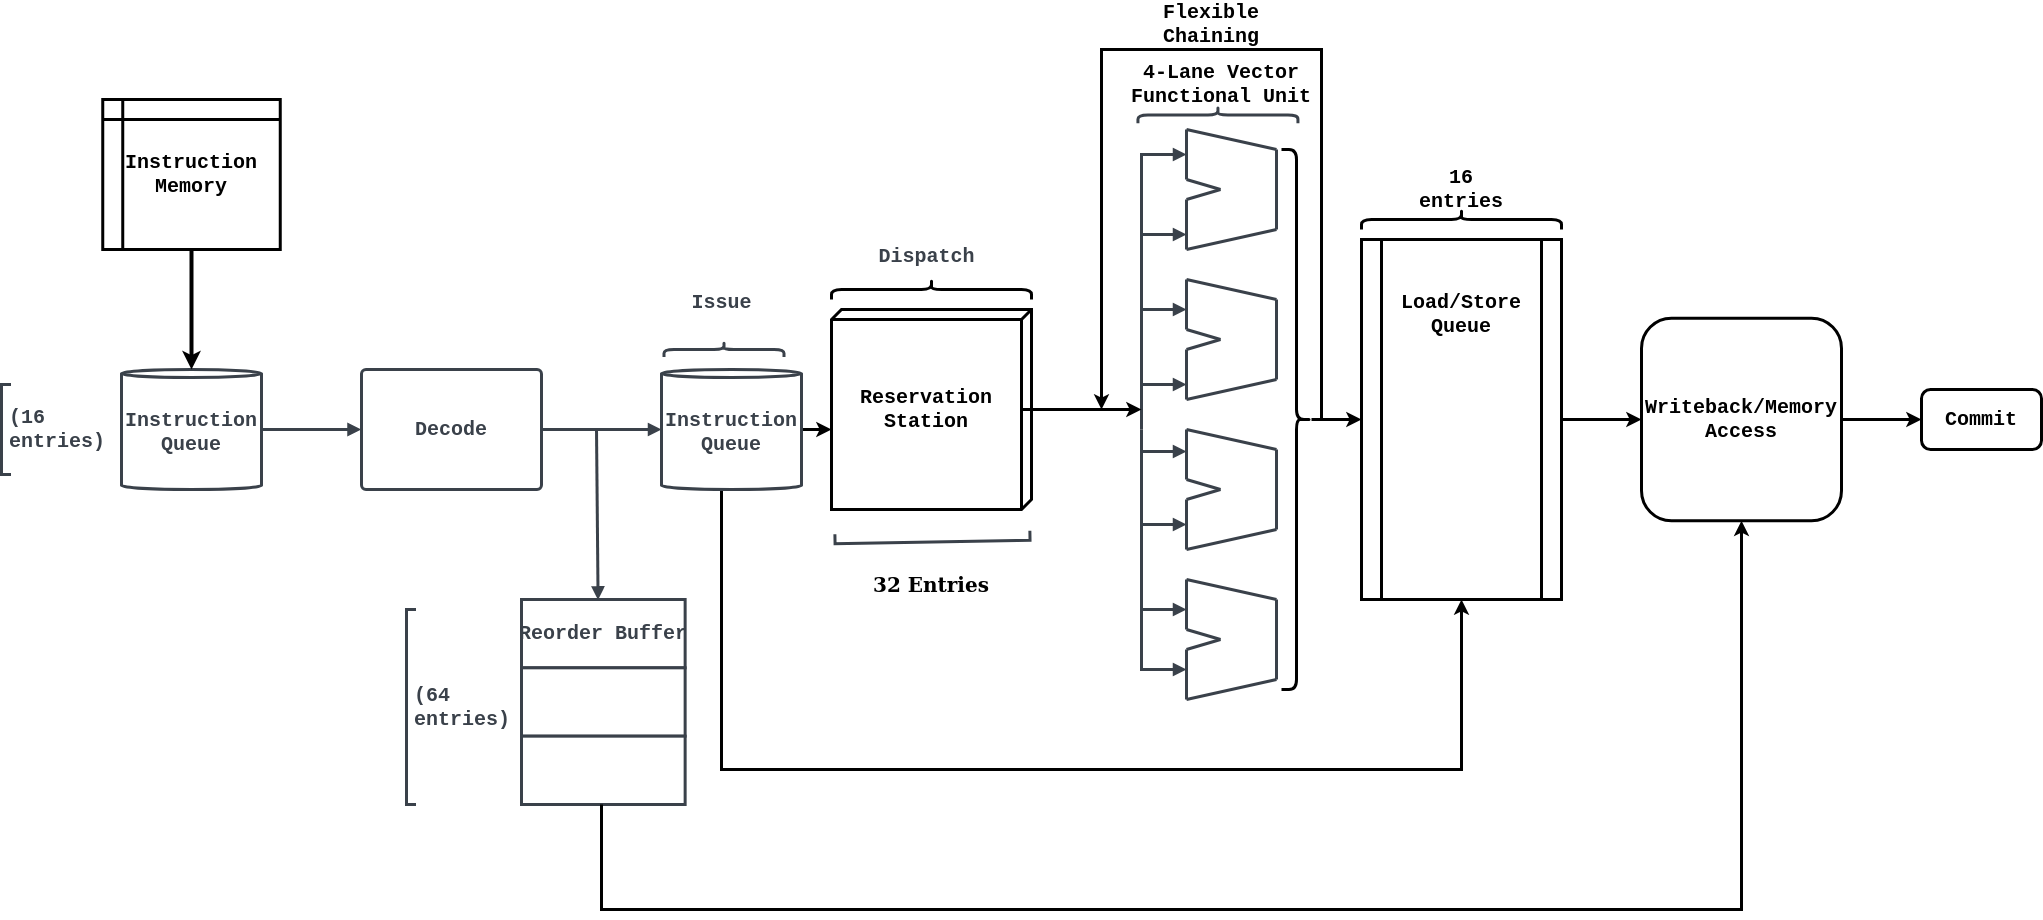
\includegraphics[scale=.135]{../abstract/diagram.png}
        \captionof{figure}{Block Diagram of proposed system's pipeline}
    \end{center}
    \begin{itemize}
        \item Fixed Length vector operands (8 elements)
        \item Out-of-Order Execution width multi-issue width(4 instructions)
        \item Reorder Buffer and Reservation Station
        \item Multi-lane execution with Chaining
    \end{itemize}
\end{frame}

% Section about generating a trace
\section{}
% Acknowledgements or Conclusion Slide
\begin{frame}{SIMD Trace}
    \begin{itemize}
        \item Using Intel's Pin tool to dynamically analyze a running binary
        \item Profiled AVX/AVX2 instructions to collect vector
            instructions
        \item Scalar instructions are excluded since vector architecures only handle
            vector instructions.
    \end{itemize}
    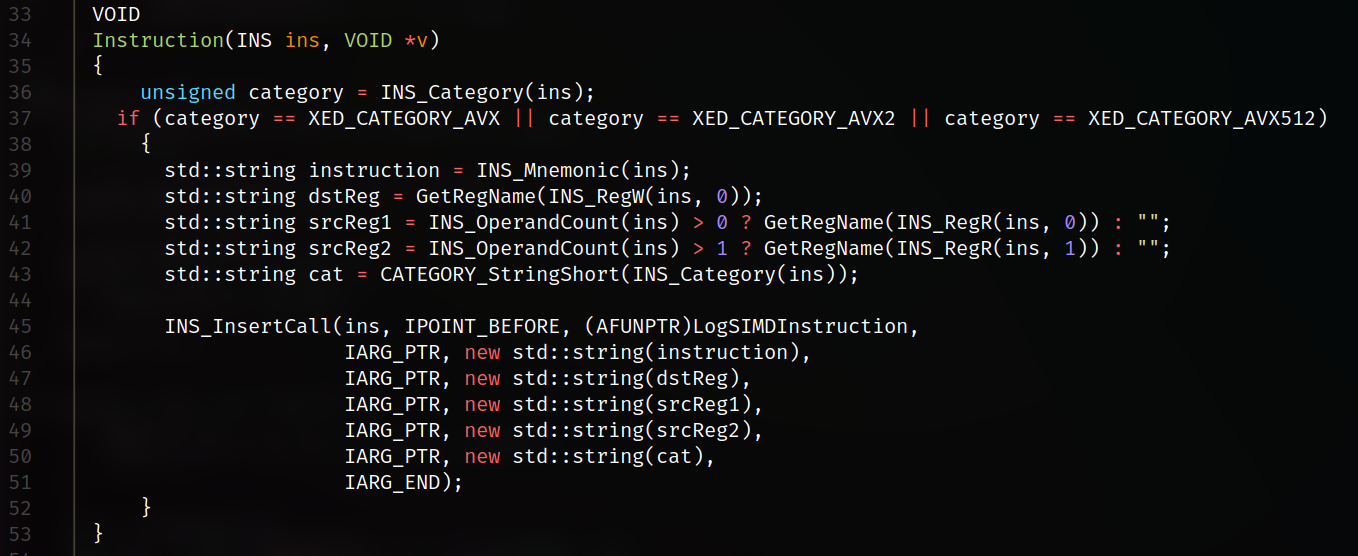
\includegraphics[scale=.3]{pin_snip.png}
    \captionof{figure}{Written pin tool to filter intel Vector instructions}
\end{frame}
\subsection{Simulator Details}
\begin{frame}{SIMD Trace}
    \begin{columns}[T]
        \begin{column}{0.7\textwidth}
            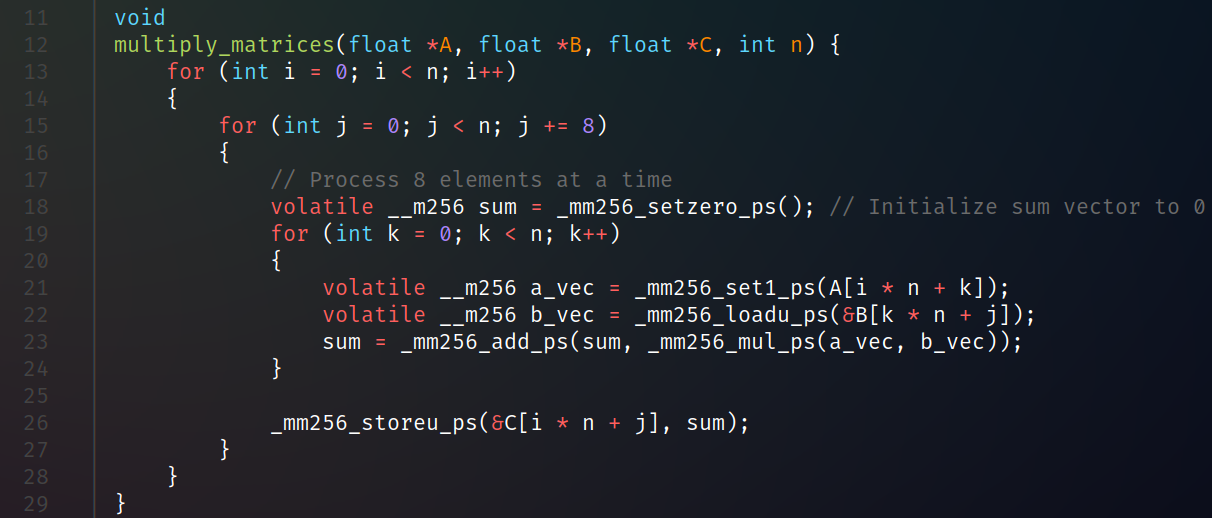
\includegraphics[scale=.225]{mm.png}\\
            \captionof{figure}{C program utilizing AVX intrinsics}
        \end{column}
        \begin{column}{0.5\textwidth}
            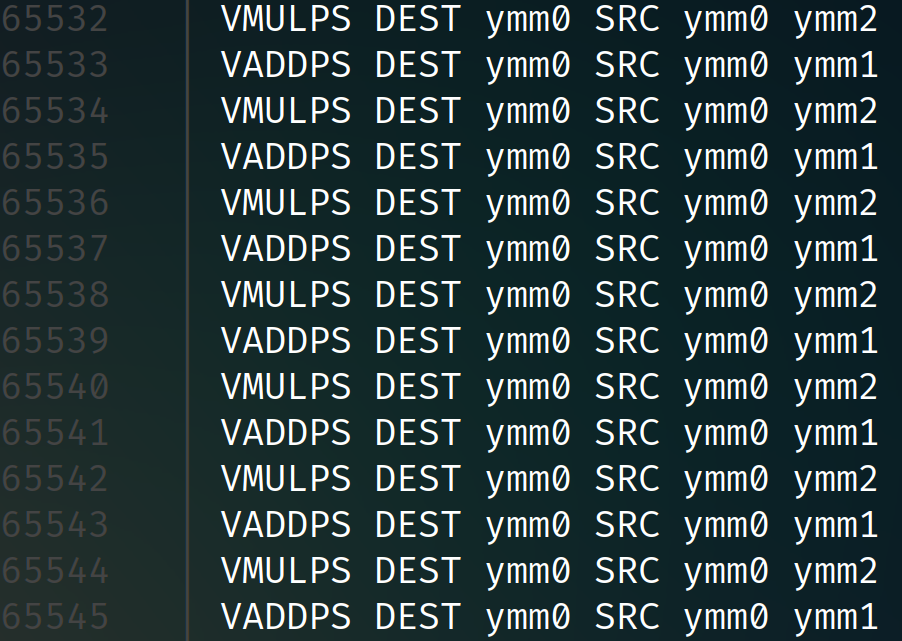
\includegraphics[scale=.2]{trace.png}
            \captionof{figure}{trace file generated}
        \end{column}
    \end{columns}
    \begin{itemize}
        \item Will assume a latency of 2 cycles for the vector addition and 8 cycles
            for vector multiplication (latency applied to each execution unit)
        \item Will entire vector data is loaded simultaneously
        \item Simulator will vary the amount of lanes in each set of execution units, but 
            will not be bottlenecked by the amount of units
    \end{itemize}
\end{frame}

\section{Goals \& Challenges}
\begin{frame}{Goals \& Challenges}
    \textbf{Goals}
    \begin{itemize}
        \item Vary lane amount to see how average IPC and max IPC is affected. Will varry lanes from 
            1 to 8.
    \end{itemize}
    \textbf{Challenges}
    \begin{itemize}
        \item Writing the pipeline simulator
            \begin{itemize}
                \item Potentially challenging
            \end{itemize}
    \end{itemize}
\end{frame}

% End of the Document
\end{document}

